%________________________________________________________________________________________
% @brief    LaTeX2e Resume for Kamil K Wojcicki
% @author   Kamil K Wojcicki
% @url   http://linux.dsplabs.com.au/?p=54
% @date     Decemebr 2007
% @info     Based on Latex Resume Template by Chris Paciorek 
%        http://www.biostat.harvard.edu/~paciorek/
%________________________________________________________________________________________
\documentclass[margin,line,a4paper]{resume}

\usepackage[utf8]{inputenc} %utf8
\usepackage[english,danish]{babel}
\usepackage[T1]{fontenc}
\usepackage{graphicx,wrapfig}
\usepackage{url}
\usepackage[colorlinks=true, a4paper=true, pdfstartview=FitV,
linkcolor=blue, citecolor=blue, urlcolor=blue]{hyperref}
\pdfcompresslevel=9


\begin{document}
{\sc \Large Curriculum Vitae -- Grigorev Dmitriy}
\begin{resume}
    \vspace{0.5cm}
    \begin{wrapfigure}{R}{0.3\textwidth}
        \vspace{-1cm}
       \begin{center}
       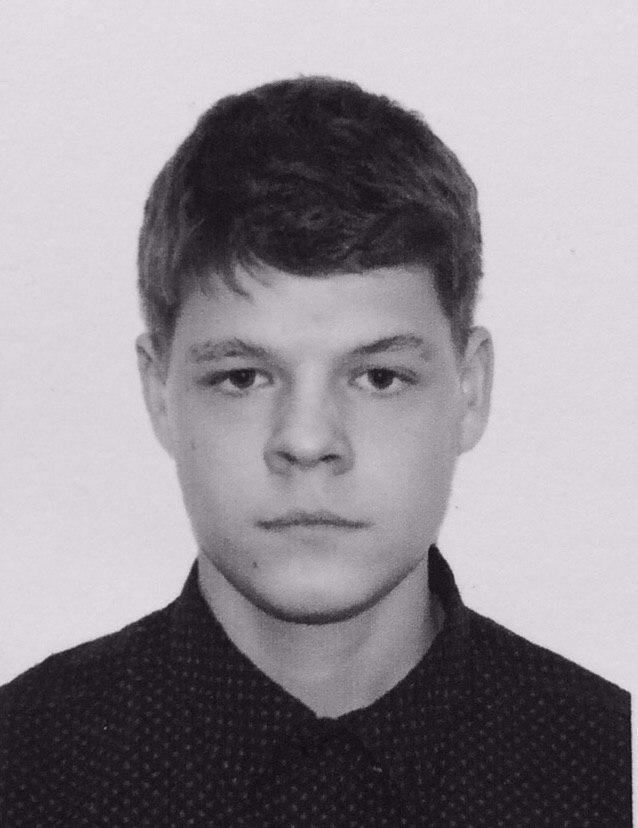
\includegraphics[width=0.3\textwidth]{mono_dima.jpg}
       \end{center}
        \vspace{-1cm}
    \end{wrapfigure}
    


    \section{\mysidestyle Personal\\Information}%\vspace{2mm}
    Grigorev Dmitriy \\
    \\
    Moscow\\
    Date of birth: 26 June, 1998\\
    tel: +79958815766 \\
    \href{mailto: skate\underline{ }9819@mail.ru}{skate\underline{ }9819@mail.ru} \\
    Occupation: engineer \\
    Status: married\\


    \section{\mysidestyle Education}

    \textbf{2016-2020} Bachalor of Applied Mathematics and Informatics in Moscow National Research University Higher School of Economics 

    \textbf{2005-2016} School N\textsuperscript{\underline{o}}2, Gus-Crystal 
    
\section{\mysidestyle Languages}
    \textbf{Russian} – Native \\
    \textbf{English} – Upper intermediate \\

\section{\mysidestyle Computer Skills}
    \textbf{Main languages}: Golang, C/C++, Python\\
    \textbf{Frameworks and Technologies}: Data science(sklearn, pandas, etc.),  System administration (Linux, Bash), Apache Kafka, Docker, Kubernetes\\
    \textbf{Basic Knowledge}: Java, Perl, PHP, Assembler, SQL, Scala, HTML\\
    
\section{\mysidestyle Job \\ experiences}
    \textbf{2021 Joom, as a software engineer} \\
    I worked in the client backend team. Our team was responsible for the backend of the entire client logic of the application and the site. The shopping cart, the display of product cards on the marketplace, the user's personal account, sales and promotions - all this was done by our team. Now I work in the JoomPro department (b2b orders from China), our team is engaged in a service for convenient administration of all orders. I'm writing code in Golang. \par
    \textbf{2020 Avito, as a software engineer} \\
    Worked in the communications department. Our services were responsible for all calls to Avito, for their security. On the website, we did not display the real number of the client, but gave a replacement number, when calling to which we redirected to the real number, recorded all these calls. They also engaged in the personal account of big sellers on Avito, where they could track all calls, listen to the recording and see which manager they called. We worked with all major telephone companies, rented replacement numbers from them and worked with their API. I wrote code in Golang, PHP. \par 
    \textbf{2018 Tinkoff, as a software engineer} \\
    I worked in the data flow management team, we were organizing all the work of the "kafka" message broker. Almost all the data that was in the bank passed on our servers. I was responsible for the stable and continuous operation of our servers, as well as for the entire infrastructure around "kafka". I wrote code in Golang, python. \par
    \textbf{2018 Yandex, as a software engineer intern} \\
    I worked in the search robot team. We developed map-reduce that processed all the information in a huge amount, aggregated it in order for the search to work correctly. The spider (the so-called robot that walks all over the Internet) sent us all the data that it collected all over the Internet, and we processed them. I wrote in C++, python and a bit of Perl. \par
    \textbf{2017-2018 Teacher of programming in the  Association of Olympic Winners} \\


\section{\mysidestyle Awards}
    \textbf{2018:} Diploma of the third degree in XIX Open All-Siberian Olympiad(ACM rules) in Programming named after I.V. Pottosin\\
    \textbf{2016:} Diploma of the second degree of Olympiad in informatics named after Lomonosov\\
    \textbf{2015-2016:} Winner of the regional stage of the All-Russian Olympiad in programming\\
    \textbf{2014:} Prize-winner of the regional stage of the All-Russian Olympiad in programming\\
\end{resume}
\end{document} 
